%
% $Id: $
%
%
% Compilar a .pdf con LaTeX (pdflatex)
% Es necesario instalar Beamer (paquete latex-beamer en Debian)
%

%
% Gráficos:
% Los gráficos pueden suministrarse en PNG, JPG, TIF, PDF, MPS
% Los EPS deben convertirse a PDF (usar epstopdf)
%

\documentclass[17pt,aspectratio=169]{beamer}
\usetheme[orchid]{Hannover}
%\usebackgroundtemplate{
\includegraphics[width=\paperwidth]{format/libresoft-bg-soft.png}}
\usepackage[spanish]{babel}
\usepackage[utf8]{inputenc}
\usepackage{graphics}
\usepackage{amssymb} % Simbolos matematicos
\usepackage{transparent}

%\definecolor{libresoftgreen}{RGB}{162,190,43}
%\definecolor{libresoftblue}{RGB}{0,98,143}

%\setbeamercolor{titlelike}{bg=libresoftgreen}

%% Metadatos del PDF.
%% \hypersetup{
%%   pdftitle={La tecnología no es neutra},
%%   pdfauthor={Jesús M. González Barahona},
%%   pdfcreator={GSyC/LibreSoft, Universidad Rey Juan Carlos},
%%   pdfproducer=PDFLaTeX,
%%   pdfsubject={},
%% }
%%

\newcommand\YUGE{\fontsize{48}{60}\selectfont}

\AtBeginSection[]
{
  {
    \usebackgroundtemplate{\hbox to \paperwidth{\hfil{\transparent{0.7}\includegraphics[width=\linewidth,height=\paperheight]{\secimage}}}}
    \begin{frame}<beamer>

      \begin{center}
        {\YUGE\bf\insertsection}
      \end{center}
    \end{frame}
  }
  \renewcommand{\secimage}{figs/bookpages}
}

% Pixbay
% NikolayFrolochkin
% https://pixabay.com/en/book-reading-library-literature-1261800/
% License: CC0 Creative Commons
\newcommand{\secimage}{figs/bookpages}

\begin{document}

\title{El sentido del software libre en la educación}
%\subtitle{}
\author{Jesús M. González Barahona}
\institute{Correo: jgb@gsyc.es ~~~~ Twitter: @jgbarah2 \\
  Universidad Rey Juan Carlos \\ }

\date{Jornadas 2019 MAX 10.0 \\
  Madrid, 10 de mayo de 2019 \\
{\small \url{https://jgbarah.github.io/presentations}} \\}

\frame{
\maketitle
}
%% \begin{center}
%% 
\includegraphics[width=6cm]{format/gsyc-urjc}
%% \end{center}

%% \begin{frame}

%%   {\Large
%%     \tableofcontents
%%   }

%% \end{frame}


% Public Domain Files (Open Clip Art Library)
% Petr Kratochvil
% http://www.publicdomainfiles.com/show_file.php?id=13953460816741
% License: Public Domain
\renewcommand{\secimage}{figs/ordenador-bebe}


%%---------------------------------------------------------------
%%---------------------------------------------------------------
\section{Ordenadores, ordenadores}


%%---------------------------------------------------------------

\begin{frame}
\frametitle{El ordenador, esa máquina maravillosa...}

Una herramienta posibilitadora:

\begin{itemize}
\item Permite realizar cualquier cosa que pueda hacer un programa
\item ...y los programas pueden hacer muchas cosas
\end{itemize}


\end{frame}

%%---------------------------------------------------------------

\begin{frame}
\frametitle{El ordenador, esa máquina maravillosa...}

Pero además...

\begin{itemize}
\item ...podemos instalar cualquier programa
\item ...podemos construir cualquier programa
\item ...podemos compartir cualquier programa
\item (o convencer a alguien para que lo construya)
\end{itemize}

\vspace{.2cm}

\begin{center}
Software y ordenador: conocimiento en acción
\end{center}
\end{frame}

%%---------------------------------------------------------------

\begin{frame}
\frametitle{...a la que imponemos limitaciones}

Pero se acepta que los programas vengan ``limitados'':

\vspace{.2cm}

\begin{itemize}
\item Limitaciones al uso
\item Limitaciones al entendimiento
\item Limitaciones a la distribución
\item Limitaciones a la modificación
\end{itemize}

\end{frame}

%%---------------------------------------------------------------

\begin{frame}

\begin{center}
\textbf{\Huge ¿Por qué aceptamos estas limitaciones?}
\end{center}
\end{frame}

% Wikimedia Commons
% Gregor Richards
% https://commons.wikimedia.org/wiki/File:Free_Software_and_Open_Source_Software_Composite_Logo.svg
% License: Creative Commons Attribution 3.0 Unported, Creative Commons Attribution-ShareAlike 2.0
\renewcommand{\secimage}{figs/software-libre}

%%---------------------------------------------------------------
%%---------------------------------------------------------------
\section{Software libre}

%%---------------------------------------------------------------

\begin{frame}
\frametitle{Algunos visionarios cambiaron el mundo}

A principios de los 1980s hubo quien se hizo esta pregunta...

\vspace{.1cm}

...y se propuso mostrar cómo el software libre nos empodera.

\vspace{.1cm}

Las implicaciones son enormes

\begin{flushright}
{\small \url{http://www.gnu.org/philosophy/free-sw.html}}
\end{flushright}
\end{frame}

%%---------------------------------------------------------------

\begin{frame}
\frametitle{El software libre permite...}

{\large
\begin{itemize}
\item usarlo como mejor te parezca
\item redistribuirlo a quien quieras
\item modificarlo (mejorarlo, adaptarlo)
\item redistribuir las modificaciones
\end{itemize}
}
\end{frame}

%%---------------------------------------------------------------

\begin{frame}
\frametitle{Consecuencias}

\begin{itemize}
\item Cualquiera tiene acceso al conocimiento \\
  ...adaptar, modificar, innovar incrementalmente
\item Cualquiera tiene acceso a la herramienta \\
  ...utilizarla para sus fines
\item Cualquiera puede colaborar \\
  ...comunidades de innovación
\end{itemize}

\end{frame}


%% ---------------------------------------------------------------

\begin{frame}
\frametitle{Y la realidad cambió...}

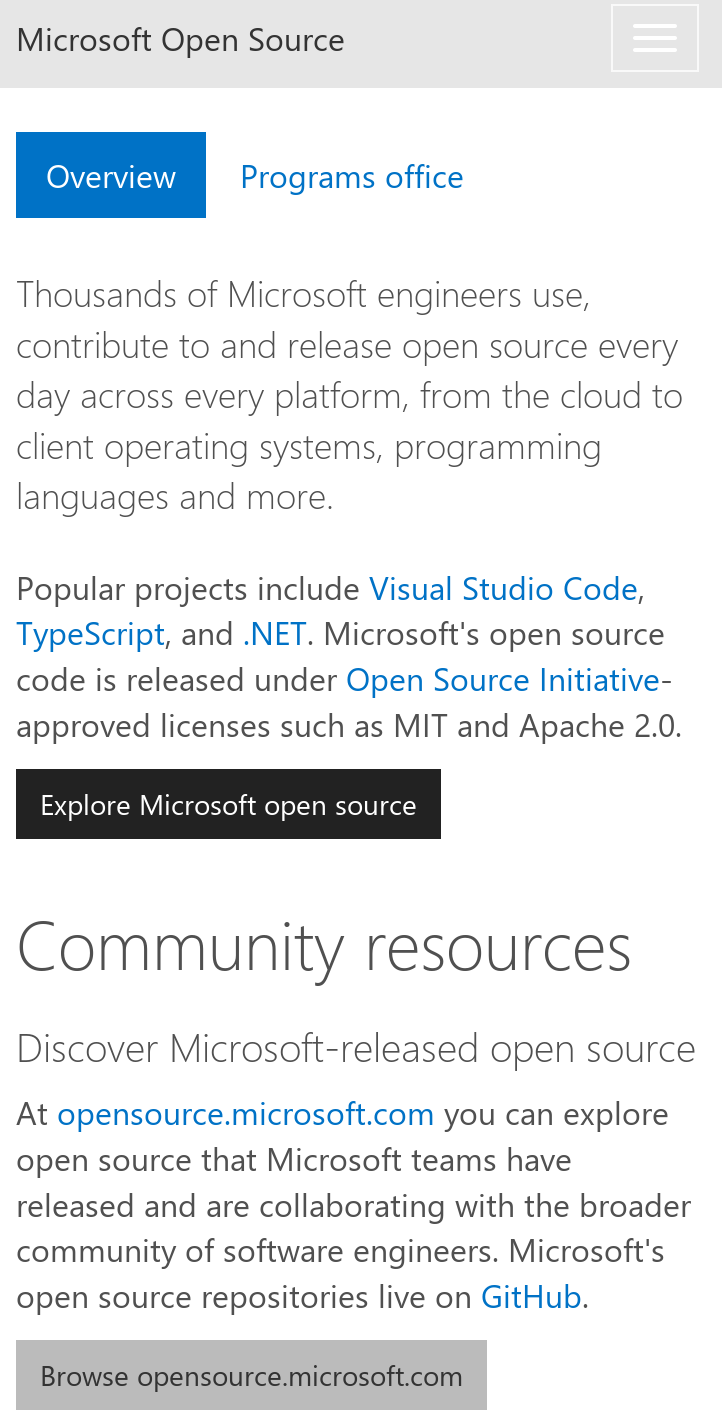
\includegraphics[width=.3\linewidth]{figs/microsoft-opensource}
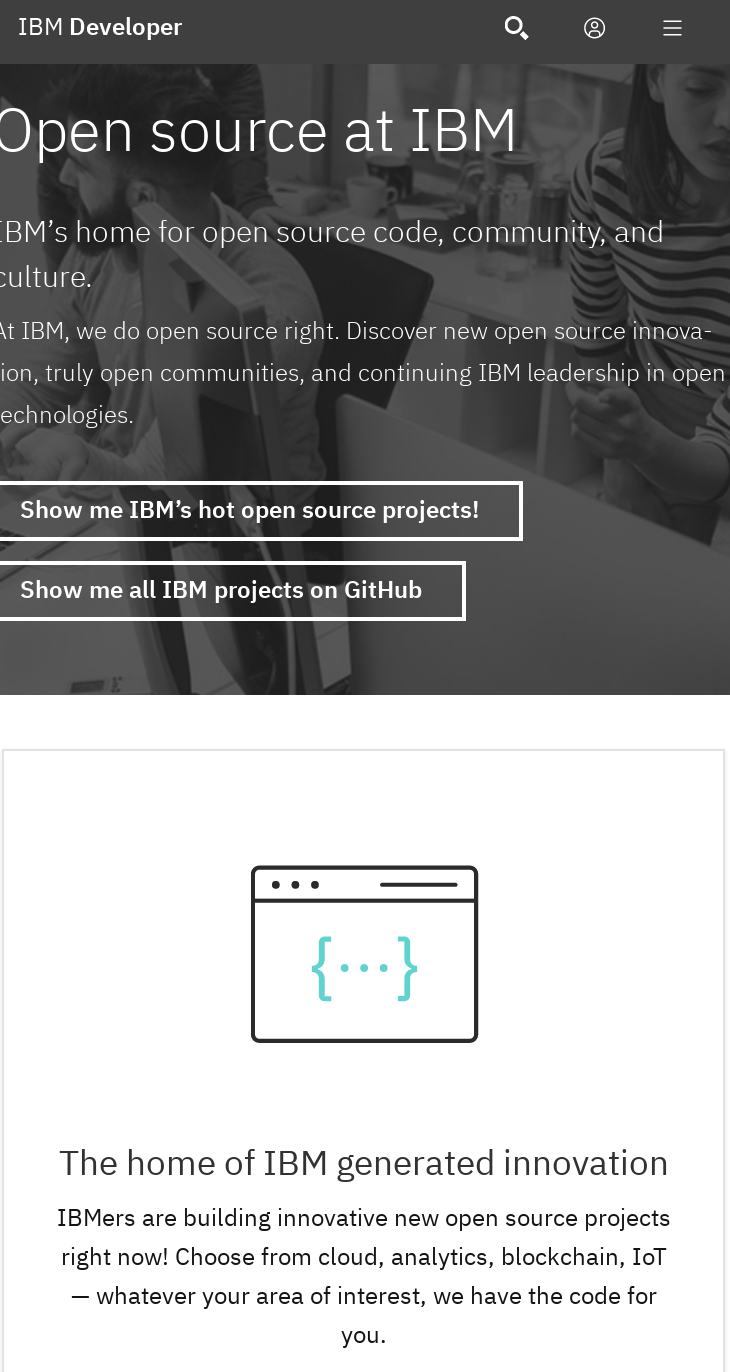
\includegraphics[width=.3\linewidth]{figs/ibm-opensource}
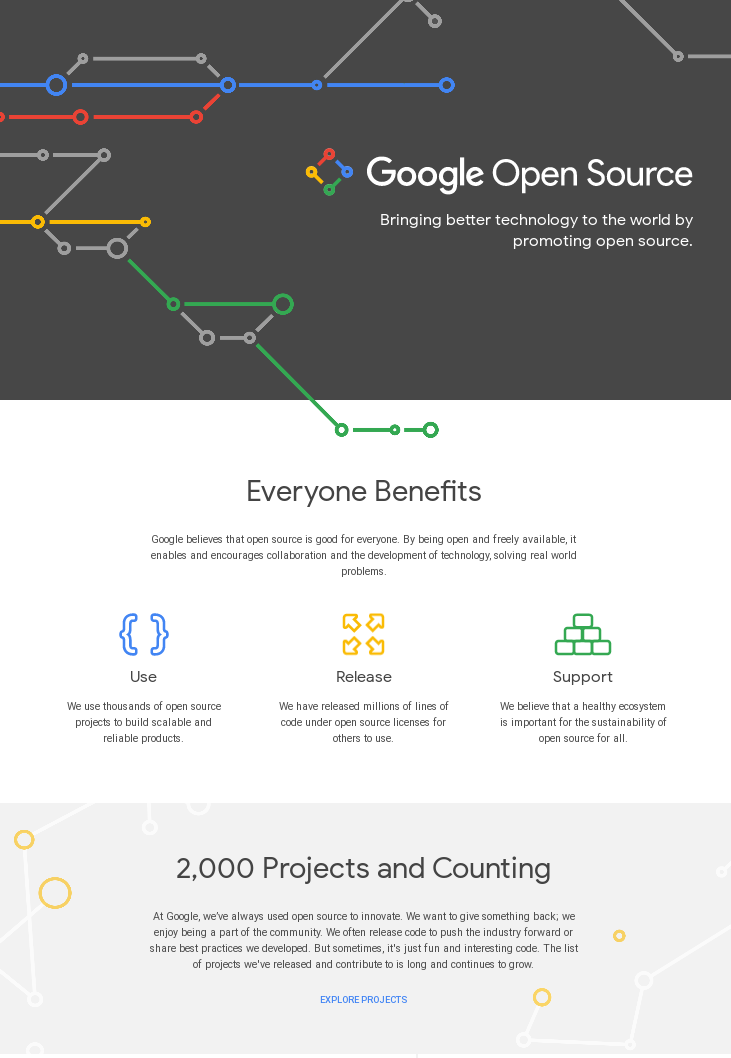
\includegraphics[width=.3\linewidth]{figs/google-opensource}

\end{frame}

%%---------------------------------------------------------------

\begin{frame}
\frametitle{Y la realidad cambió...}

{\Large
\begin{center}
  El software libre \\
  es la infraestructura \\
  verdaderamente común \\
  de la \\
  sociedad de la información \\
\end{center}
}
\end{frame}

%%---------------------------------------------------------------
%%---------------------------------------------------------------
\section{Software libre y educación}

%%---------------------------------------------------------------

\begin{frame}
\frametitle{Nuevas posibilidades}

\begin{itemize}
  \item Reproducir
\item Adaptar
\item Explorar
\item Compartir
\item Enfocar
\end{itemize}

\end{frame}

%%---------------------------------------------------------------

\begin{frame}
\frametitle{Reproducir}

\begin{itemize}
\item Es facil reproducir el entorno docente
\item ...a muy bajo coste...
\item ...sin negociar con proveedores
\end{itemize}

\begin{flushright}
  Alumnos \\
  Profesores \\
  Otros centros \\
  Cualquier persona... \\
\end{flushright}
\end{frame}

%%---------------------------------------------------------------

\begin{frame}
\frametitle{Reproducir}

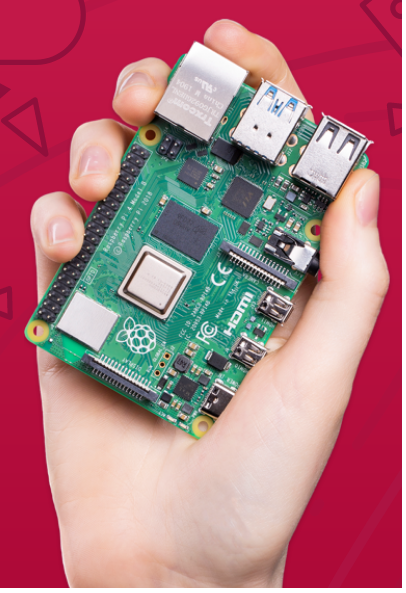
\includegraphics[width=\linewidth]{figs/raspberry-pi}

\begin{flushright}
\href{https://raspberrypi.org/education}{raspberrypi.org/education}
\end{flushright}

\end{frame}

%%---------------------------------------------------------------

\begin{frame}
\frametitle{Adaptar}

\begin{itemize}
\item Se puede adaptar...
\item ...se puede ``pulir''...
\item ...se puede combinar
\end{itemize}

\begin{flushright}
  Idiomas y usos lingüísticos \\
  Capacidades diferentes \\
  Métodos y programas docentes \\
  Niveles educativos \\
\end{flushright}
\end{frame}

%%---------------------------------------------------------------

\begin{frame}
\frametitle{Explorar}

\begin{itemize}
\item Uso marginal de herramientas
\item Rápido ciclo de prueba / evaluación
\item Menos barreras al cambio de herramienta
\end{itemize}

\begin{flushright}
  Más flexible \\
  Más rápido \\
  Más fácil
\end{flushright}
\end{frame}

%%---------------------------------------------------------------

\begin{frame}
\frametitle{Explorar}

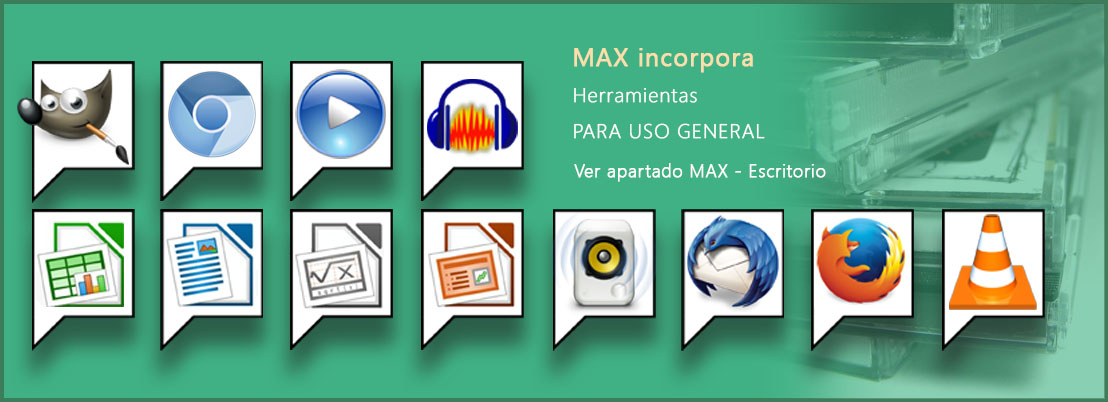
\includegraphics[width=\linewidth]{figs/max-1}

\end{frame}

%%---------------------------------------------------------------

\begin{frame}
\frametitle{Explorar}

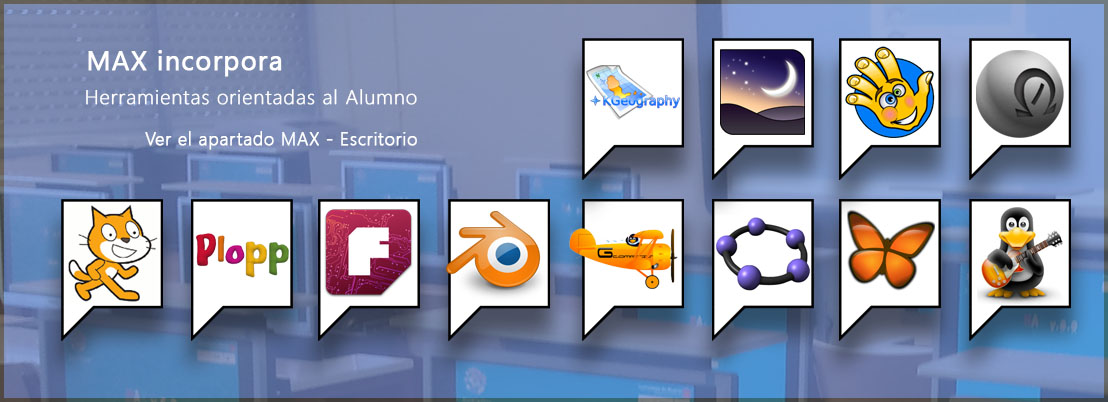
\includegraphics[width=\linewidth]{figs/max-2}

\end{frame}

%%---------------------------------------------------------------

\begin{frame}

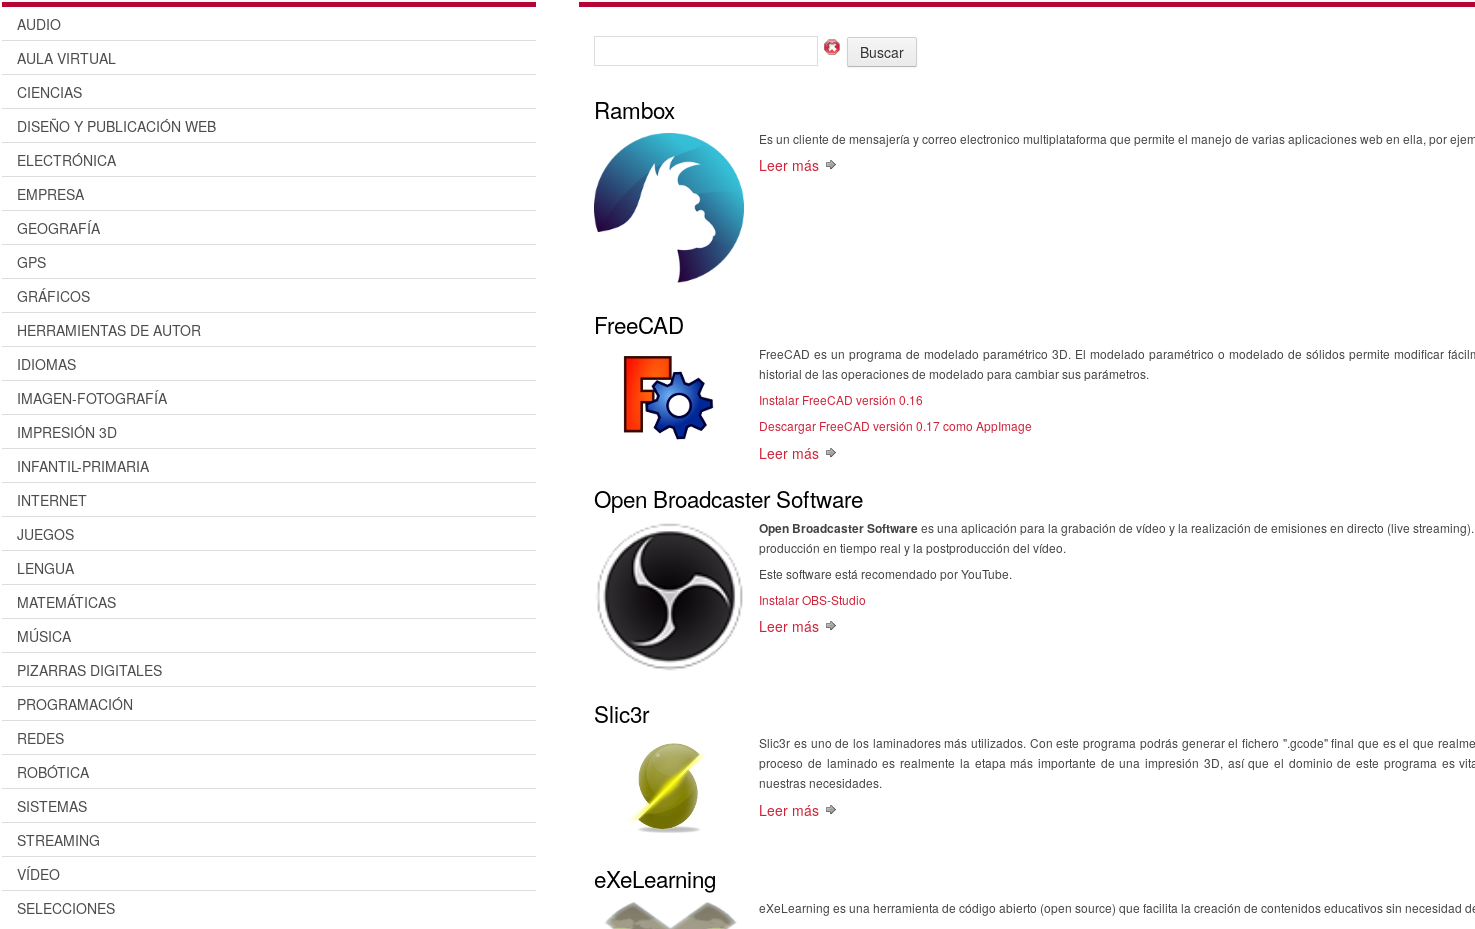
\includegraphics[width=\linewidth]{figs/max-3}

\end{frame}

%%---------------------------------------------------------------

\begin{frame}
\frametitle{Compartir}

\begin{itemize}
\item ...tus cambios
\item ...tus experiencias
\item ...tus adaptaciones
\end{itemize}

\begin{flushright}
  Rentabilidad: \\
  cualquiera puede aprovechar lo compartido \\
\end{flushright}
\end{frame}

%%---------------------------------------------------------------

\begin{frame}
\frametitle{Enfocar}

\begin{itemize}
\item Enseñar, no prescribir proveedores
\item Minimizar la gestión de licencias
\item Empoderar al educador
\item Empoderar al alumno
\end{itemize}

\begin{flushright}
  El foco puede ser la educación \\
  no el contexto comercial \\
\end{flushright}
\end{frame}


%%---------------------------------------------------------------

\begin{frame}
\frametitle{Nuevas posibilidades}


{\Huge
\begin{center}
Libertad
\end{center}
}

\end{frame}

%%---------------------------------------------------------------

\begin{frame}
\frametitle{Nuevas posibilidades}


{\Large
\begin{center}
Y no solo con software \\
también están los recursos libres \\
\end{center}
}

\end{frame}

% Pixbay
% djedj
% https://pixabay.com/es/photos/spiderman-maravilla-hero-super-hero-3309033/
% License: Pixabay

%%---------------------------------------------------------------

\begin{frame}

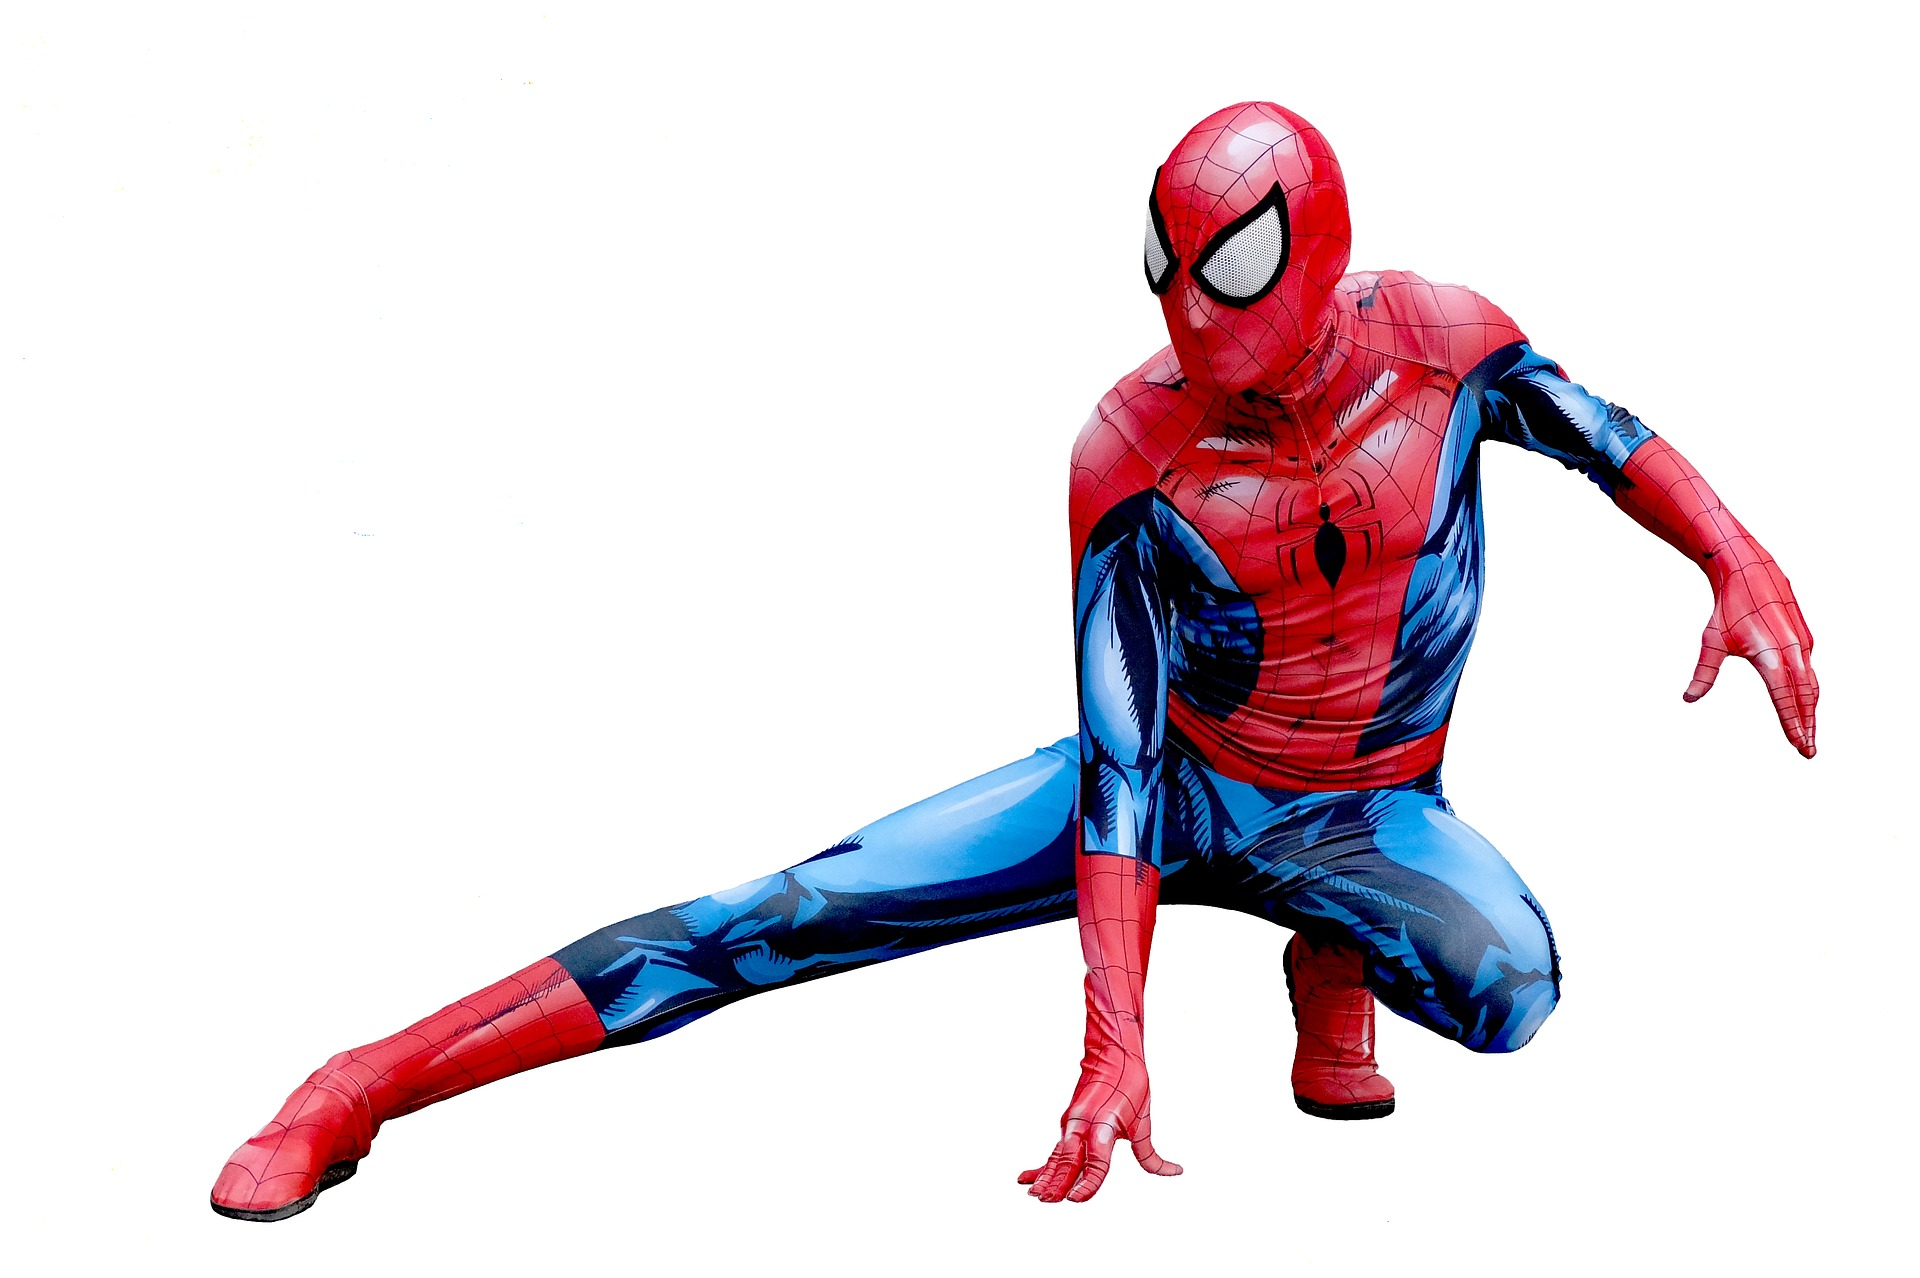
\includegraphics[height=.7\textheight]{figs/spiderman.jpg}

{\Large
\begin{center}
  Un gran poder conlleva \\
  una gran responsabilidad \\
\end{center}
}

\end{frame}

%%---------------------------------------------------------------

\begin{frame}
\frametitle{Nuevas responsabilidades}

\begin{itemize}
\item Nuevas habilidades, capacidades
\item Nuevos hábitos
\item Nuevas tareas
\item Nuevas necesidades
\end{itemize}

\end{frame}

%%---------------------------------------------------------------

\begin{frame}
\frametitle{Habilidades, capacidades}

\begin{itemize}
\item El software es una herramienta docente más
\item Instalar, probar, no es para otros
\item Programar es para todos
\end{itemize}

\begin{flushright}
  Los tiempos cambian \\
  Las herramientas también \\
\end{flushright}
\end{frame}


%%---------------------------------------------------------------

\begin{frame}

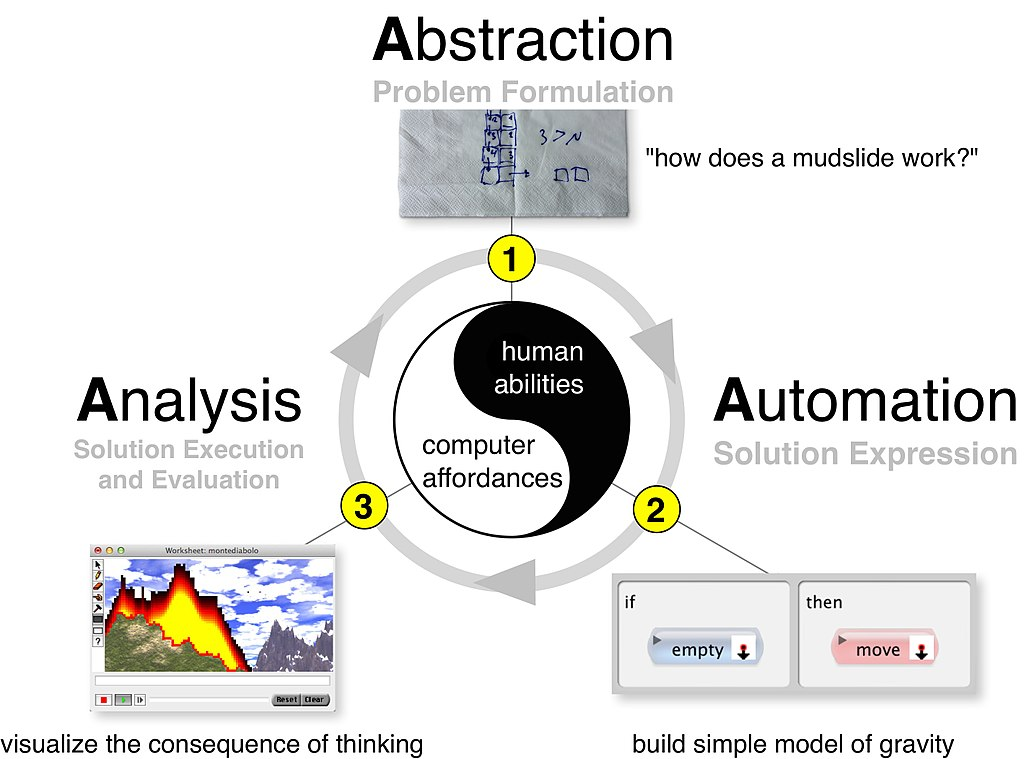
\includegraphics[height=\textheight]{figs/computational-thinking}
\end{frame}


%%---------------------------------------------------------------

\begin{frame}
\frametitle{Hábitos}

\begin{itemize}
\item Probar opciones
\item Aprender para ir un paso por delante
\item Organizarse
\item Colaborar
\end{itemize}

\begin{flushright}
  ¡¡Creatividad al poder!!
\end{flushright}
\end{frame}

%%---------------------------------------------------------------

\begin{frame}
\frametitle{Tareas}

\begin{itemize}
\item Vigilar programas interesantes
\item Repensar las asignaturas
\item Mantenerse al día
\item Integrarse en comunidades
\end{itemize}

\begin{flushright}
  Vida activa, \\
  vida sana \\
\end{flushright}
\end{frame}

%%---------------------------------------------------------------

\begin{frame}
\frametitle{Necesidades}

\begin{itemize}
\item Tiempo
\item Formación
\item Apoyo experto
\item Planificación institucional
\end{itemize}

\begin{flushright}
  Las herramientas son sólo herramientas \\
  hay que poder manejarlas \\
\end{flushright}
\end{frame}


% Tip Jar, Alamo Beer
% Nan Palmer
% Wikimedia Commons
% https://commons.wikimedia.org/wiki/File:Tip_Jar,_Alamo_Beer_(2015-03-26_18.48.31_by_Nan_Palmer).jpg
% License: Creative Commons Attribution 2.0 Generic
\renewcommand{\secimage}{figs/tipjar}
{\bf
  \textcolor[rgb]{1,1,1}{
    \section{Propina}
  }
}

%%---------------------------------------------------------------

\begin{frame}
\frametitle{Documentación libre}

\begin{itemize}
\item Del software a los materiales docentes \\
  (apuntes, libros, manuales, vídeos, audios)
\item Licencias libres
\item Apoyo de herramientas (ej: wiki)
\item Primeros pasos en gran escala: \\
  OpenCourseWare (MIT), Wikipedia
\end{itemize}

{\Large
\begin{center}
Idea: libros libres para asignaturas
\end{center}
}

\end{frame}

%%---------------------------------------------------------------
% LICENCIA DE REDISTRIBUCION DE LAS TRANSPAS
\frame{
~
\vspace{3cm}

\begin{flushright}
{\small
\copyright 2012-2019 Jesús M. González Barahona. \\

  Algunos derechos reservados. \\
  Este artículo se distribuye bajo la licencia \\
  ``Reconocimiento-CompartirIgual 3.0 España'' \\
  de Creative Commons, \\
  disponible en \\
}
{\footnotesize
  \url{https://creativecommons.org/licenses/by-sa/3.0/es/} \\
}
\end{flushright}
}

\end{document}
